\documentclass[a4paper,12pt]{article}
\usepackage[utf8]{inputenc}
\usepackage[german, ngerman]{babel}
\usepackage{graphicx}
\usepackage[figurename=Bild]{caption}
\usepackage{inputenc}
\usepackage{geometry}


%opening
\title{Sech Anzahl grafisch darstellen}
\author{Burak Erol, Philipp Winterholler}

\begin{document}

\section{Sech Anzahl grafisch darstellen}

Um den Nutzer eine �bersicht aller gefundenen Sech-Tags grafisch darzustellen, wurde ein Label �ber den Sech-Button erg�nzt, welche die Anzahl der Sech-Tags in einer roten Schrift angibt. Diese Anzahl soll dem Nutzer zeigen, wie viele Sech-Tags sich auf der Webseite befinden. Beim bedienen des Sech-Buttons, wird die Sech-Tabelle animiert. Diese Tabelle wird rechts im -Browser ein- und ausgefahren. Das WK-Webview wird dementsprechend vergr��ert oder verkleinert. Bedient man diesen Sech-Button, so klappt sich eine Tabelle vom rechten Bildschirm aus und liefert alle Tags in einer TableView zur�ck. Diese zur�ckgelieferten Tags werden in seperaten Zellen auf der TableView abgespeichert, welche dem Nutzer durch anklicken eine neue Pop-Up Seite, spezifisch zu dem angeklickten Tag, �ffnet. Aufgrund der Umstellung der Navigationsleiste wird diese grafische Darstellung der Anzahl an Sech-Tags nicht mehr angezeigt. Die Umstellung der Navigationsleiste war notwendig um die H�he und Breite des WKWebViews festzulegen, darum wurde ein neuer Navigation Controller erzeugt, der die Navigation Bar schon direkt mitliefert. In diese erzeugte Navigation Bar k�nnen jedoch keine Labels beliebig positioniert werden, somit wurde diese Option ausgeblendet.


\includegraphics[width=12cm]{Pics/Sech_Anzahl}
\newpage
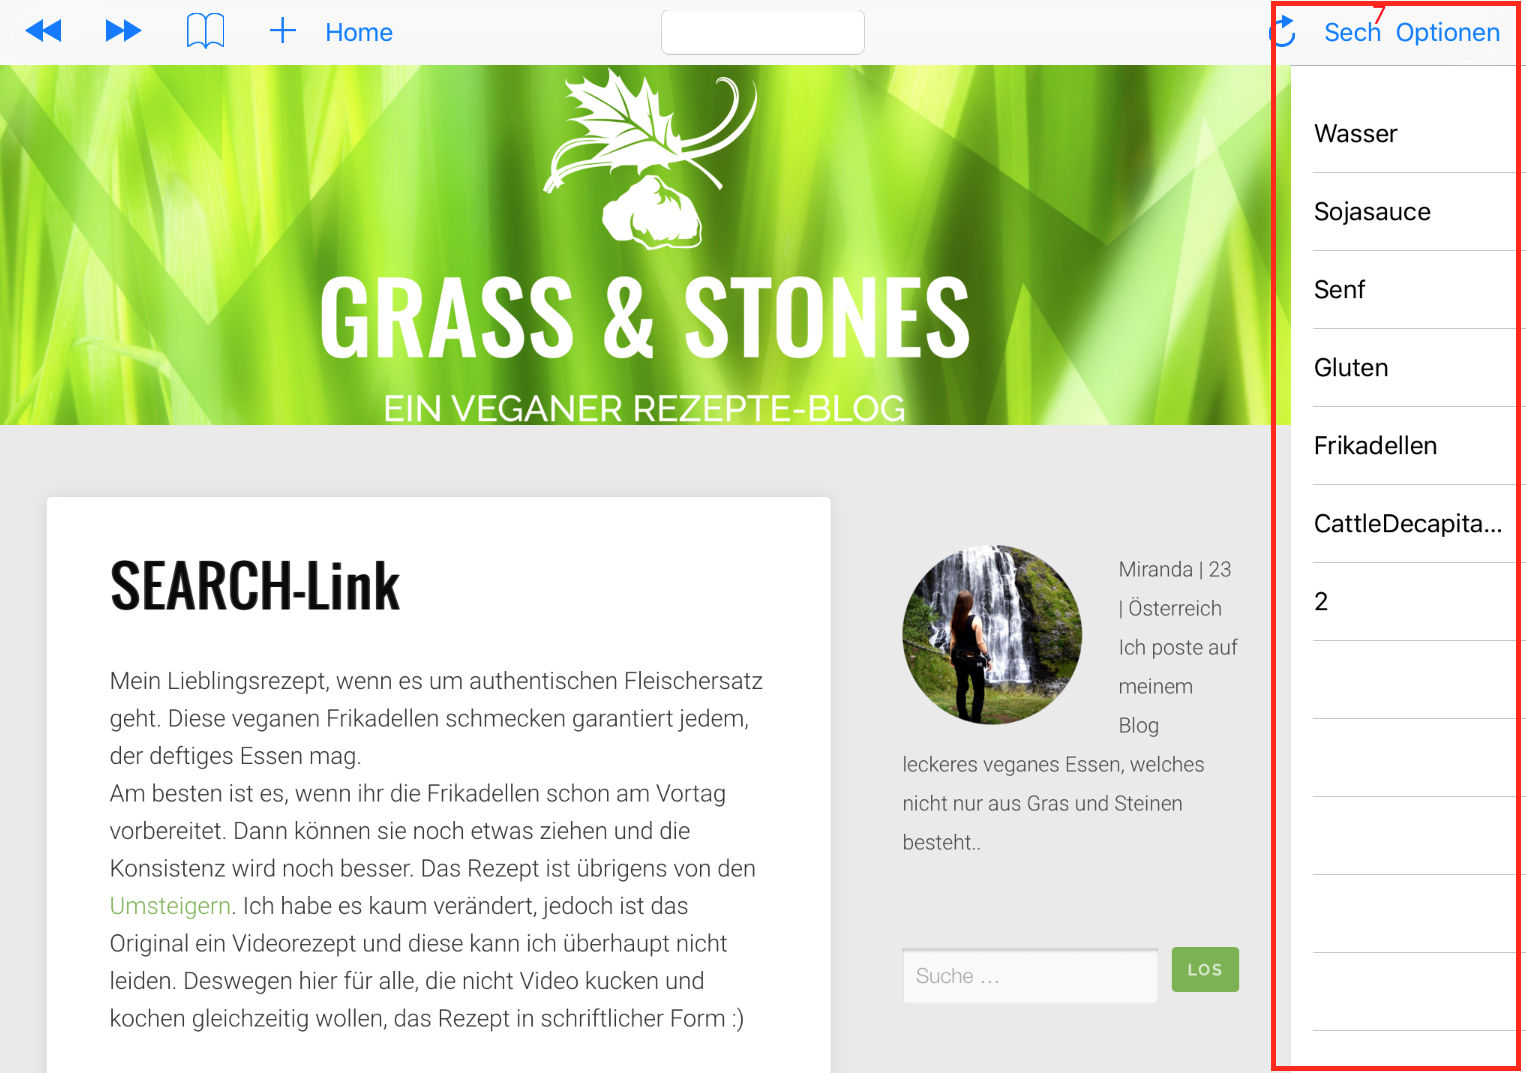
\includegraphics[width=12cm]{Pics/Sech_Tabelle_aufgeklappt}
\newpage

\includegraphics[width=12cm]{Pics/Sech_Tabelle_versteckt}

\end{document}
